\documentclass[xetex,twocolumn,epjc3]{svjour3}

% \RequirePackage[T1]{fontenc}  % 不需要，xelatex 使用 Unicode
\usepackage{fontspec}  % xelatex 字体支持
% 尝试使用 Times 字体，如果不存在则使用 Latin Modern Roman
\IfFontExistsTF{Times New Roman}{%
  \setmainfont{Times New Roman}[Ligatures=TeX]%
}{%
  \setmainfont{Latin Modern Roman}[Ligatures=TeX]%
}
\smartqed
\RequirePackage{graphicx}
% \RequirePackage{mathptmx}  % 与 fontspec 冲突
\RequirePackage{flushend}
\RequirePackage[numbers,sort&compress]{natbib}
\RequirePackage[colorlinks,citecolor=blue,urlcolor=blue,linkcolor=blue]{hyperref}
\RequirePackage{amsmath}   % 你需要数学公式就加
\RequirePackage{algorithm2e}  % 如果确实要用算法环境
\RequirePackage{subcaption}
\RequirePackage{ragged2e}
\RequirePackage[english]{babel}
\RequirePackage{microtype}
\journalname{Eur. Phys. J. C}
\newenvironment{dataavailability}{\paragraph{Data Availability Statement}}{}
\newenvironment{codeavailability}{\paragraph{Code Availability Statement}}{}

\begin{document}
\justifying

\title{High‑Performance Statistical Methods for Reactor Neutrino Oscillations}

\author{Jingqin Xue\thanksref{e1,addr1,addr2}
        \and Han Zhang\thanksref{addr1,addr2}
        \and Hongfang Shen\thanksref{addr1}
        \and Guangbao Sun\thanksref{addr1,addr3}
        \and Dian Li\thanksref{addr1,addr2}
        \and Liangqianjin Fan\thanksref{addr1,addr2}
        \and Haifeng Yao\thanksref{addr1,addr2}
        \and Liang Zhan\thanksref{addr1,addr2}
        \and Xiang Zhou\thanksref{addr3}
        \and Xuefeng Ding\thanksref{e2,addr1,addr2}
}


\thankstext{e1}{e-mail: xuejingqin@ihep.ac.cn}
\thankstext{e2}{Corresponding author: dingxf@ihep.ac.cn}

\institute{Institute of High Energy Physics, Chinese Academy of Sciences, Beijing 100049, China \label{addr1}
          \and University of Chinese Academy of Sciences, Beijing 100049, China \label{addr2}
          \and Hubei Nuclear Solid Physics Key Laboratory, School of Physics and Technology, Wuhan University, Wuhan 430072, China \label{addr3}
}

\date{Received: date / Accepted: date}

\maketitle

\begin{abstract}
\begin{justify}
We present a PyTorch-based framework for forward folded reactor neutrino spectrum fitting that accelerates the two main bottlenecks: IBD mapping and detector response, using (i) result caching, (ii) banded sparse matrices, and (iii) blocked construction of the response. On an Intel Xeon Gold 6338 CPU, these techniques reduce per-fit walltime by $\approx 7\times$ (median over 5 runs) relative to a dense, unoptimized implementation, with <$10^{-6}$ relative spectral error versus a double-precision baseline. The framework has been applied to reactor-neutrino oscillation analyses and is reusable in other neutrino experiments that rely on forward-folded energy spectra, enabling practical Feldman–Cousins coverage studies and large parameter scans at substantially lower computational cost.
\end{justify}
\end{abstract}

\section{Introduction}
\label{sec:intro}
\justifying
Neutrino oscillation is one of the major breakthroughs in particle physics, and reactor neutrino experiments have played a crucial role in precisely measuring oscillation parameters such as mixing angles and mass-squared differences. Historically, the Daya Bay experiment was the first to observe the disappearance of reactor $\overline{\nu}_e$ with a significance of 5.2$\sigma$~\cite{PhysRevLett.108.171803}, and measured $\sin^2 2\theta_{13} \approx 0.092$. Next-generation reactor neutrino experiments, such as JUNO~\cite{Abusleme2025}, aim to determine the neutrino mass ordering through high-precision energy spectrum measurements, while further improving the precision of oscillation parameters like mixing angles and mass-squared differences.

These experiments typically detect electron antineutrinos emitted from reactors via the inverse beta decay (IBD) process. The expected observable spectrum is obtained by convolving the antineutrino fluxes from various fission isotopes with the IBD cross section and the detector response function. This predicted spectrum is then compared with the observed reconstructed energy spectrum via bin-by-bin fitting to extract the oscillation parameters. The process involves detailed modeling of the reactor flux, IBD cross section, detector energy nonlinearity, and resolution effects, and requires repeated numerical integration (matrix convolution), resulting in substantial computational cost.

The Feldman–Cousins method is widely used in the particle physics community. For example, PROSPECT~\cite{PhysRevD.103.032001} and Daya Bay~\cite{PhysRevLett.133.051801} adopted the Feldman–Cousins method when searching for sterile neutrinos, where signals are weak and systematic uncertainties are significant, in order to avoid biases arising from the breakdown of Wilks’ theorem under low-statistics conditions. Similarly, NOvA~\cite{refId0} employed a profiled Feldman–Cousins construction because limited event statistics, the non-linear dependence on $\delta_{CP}$ and $\theta_{23}$, octant degeneracies, and physical parameter boundaries violate the regularity conditions of Wilks’ theorem. 

The Feldman–Cousins method requires extensive Monte Carlo simulations to accurately estimate the distribution of the test statistic and ensure proper confidence level coverage. This process involves generating tens of millions of pseudo-experiments and performing fits for each assumed parameter value, leading to a dramatic increase in computational cost. Therefore, accelerating the spectrum fitting procedure is essential for maintaining both efficiency and accuracy in statistical analyses.

Furthermore, as the number of energy bins and the number of fit parameters (including pull terms for systematic uncertainties) increase, traditional unoptimized fitting methods become increasingly time-consuming during large-scale parameter scans or pseudo-experiment generation. This creates a major bottleneck in constructing confidence intervals and conducting global fits.

To address this, researchers have proposed various optimization strategies to accelerate neutrino spectrum fitting. For instance, Ding et al. developed the GPU-based analysis framework GooStats~\cite{Ding_2018}, which significantly improves fitting performance by parallelizing large-scale matrix operations. Koch et al. introduced the ReMU toolkit, which models the detector response as a response matrix and performs ``forward projection`` of theoretical spectra into the reconstructed energy space via simple matrix multiplication~\cite{Koch2019}. In addition, techniques such as caching static computational results (e.g.precomputing and storing detector response grids) and sparse matrix storage (retaining only nonzero or significant elements) have been widely adopted in analysis frameworks to avoid redundant computations and reduce memory usage.

Inspired by these ideas, this study presents an accelerated framework for neutrino spectrum fitting based on PyTorch. We combine multiple optimization techniques, such as caching, sparse matrix representation, blocked multiplication and response matrix truncation (considering only elements within $\pm6\sigma$ of the Gaussian distribution)—to accelerate the computation of IBD differential cross-section mappings and detector energy response. Under the premise of preserving numerical accuracy, our tests demonstrate that the proposed method improves fitting speed by factors of several ($\approx 7 \times$ in our setup). Furthermore, by leveraging PyTorch, we achieve parallel computation on both CPU and GPU platforms.



\section{Expected spectrum calculation}
\label{sec:intro}

\subsection{Detection of reactor antineutrinos}
\label{sec:theory}
In reactor-based neutrino experiments, electron antineutrinos ($\overline{\nu}_e$) with energies in the range of a few mega-electronvolts (MeV) are primarily detected via the Inverse Beta Decay (IBD) process:  
\begin{equation}   
    \begin{aligned}  
    \label{eq:ibd} 
\overline{\nu}_e + p \rightarrow e^+ + n 
    \end{aligned}
\end{equation}
This reaction typically occurs in liquid scintillator (LS) detectors, where an antineutrino interacts with a free proton in the detector medium, producing a positron and a neutron. The positron promptly deposits its kinetic energy through ionization and subsequently annihilates with an electron, emitting two 511 keV gamma rays—collectively forming the so-called ``prompt signal``. The neutron, after thermalization, is captured by a nearby nucleus and emits characteristic gamma rays, resulting in a delayed signal on the order of hundreds of microseconds. The time and spatial coincidence of the prompt and delayed signals provides strong suppression of uncorrelated background events such as natural radioactivity and cosmogenic particles. As a result, the IBD channel is widely adopted in reactor neutrino experiments and is particularly effective for precision measurements and oscillation studies of reactor antineutrinos.

\subsection{Prediction of reactor antineutrino flux}
\label{sec:Arrived neutrino spectrum}
The electron antineutrinos ($\overline{\nu}_e$) emitted from a nuclear reactor originate from the fission of fuel isotopes, primarily $^{235}$U, $^{238}$U, $^{239}$Pu, and $^{241}$Pu~\cite{Ma2013EnergyRelease}. Based on the reactor’s thermal power and the fission fractions of these isotopes, the Huber–Mueller model is employed to predict the $\overline{\nu}_e$ energy spectra for each fissile isotope. These individual spectra are then combined using the average energy released per fission to yield the total emitted spectrum from the reactor core~\cite{Huber2011, Mueller2011}. The emitted spectrum is further modified by the electron antineutrino survival probability $P_{ee}(E_{\overline{\nu}_e}, L)$, which accounts for neutrino oscillations and matter effects arising during propagation through the Earth's crust. This results in the predicted $\overline{\nu}_e$ spectrum arriving at the detector. As shown in Fig.~\ref{fig:reactor_nu_arrival}, the inclusion of oscillation effects introduces energy-dependent oscillatory features in the spectrum, reflecting the mixing between neutrino flavor and mass eigenstates and their coherent evolution during propagation.

\subsection{Deposited energy spectrum}  
\label{sec:Deposited energy spectrum}
In the inverse beta decay (IBD) process (see section~\ref{sec:theory}), only antineutrinos with energy exceeding the threshold of approximately 1.806 MeV can initiate this reaction~\cite{Ludhova2023JUNO}. The resulting positron carries away nearly all of the incident neutrino energy, minus the 1.293 MeV proton–neutron mass difference. After annihilation, the energy deposited by the positron in the scintillator is approximately $E_{\rm dep} \approx E_{\overline{\nu}_e} - 0.8$ MeV.  The deposited-energy spectrum is obtained by folding the incoming reactor flux with the IBD differential cross section and integrating over neutrino energy:

\begin{equation}
\label{eq:continuous_rate}
\phi(E_{\rm dep}) \;=\; N_p \,  \int_{1.8}^{13} dE_{\overline{\nu}_e}\; \phi(E_{\overline{\nu}_e}) \; \frac{{\rm d}\sigma}{{\rm d}E_{\rm dep}}(E_{\overline{\nu}_e}, E_{\rm dep})  \; 
\end{equation}
\noindent where $N_p$ is the number of target protons, $\phi(E_{\overline{\nu}_e})$ is the incident antineutrino flux. The differential cross section with respect to the deposited energy is given by

\begin{equation}
\begin{split}
\frac{{\rm d}\sigma}{{\rm d}E_{\rm dep}}(E_{\overline{\nu}_e}, E_{\rm dep}) \;=
\int_{-1}^{1} {\rm d}\cos\theta \;  
\frac{{\rm d}\sigma}{{\rm d}\cos\theta}(E_{\overline{\nu}_e},\cos\theta) \\ \;  
\times \delta\!\Big(E_{\rm dep}-T_e(E_{\overline{\nu}_e},\cos\theta)-m_e\Big)
\end{split}
\end{equation}


\noindent where $E_{\overline{\nu}_e}$ is the incident antineutrino energy, $T_e$ is the positron kinetic energy, and $m_e$ is the electron mass. This expression represents the mapping from the neutrino energy and scattering angle to the observable deposited energy $E_{\rm dep}$. And $d\sigma/d\cos\theta$ denotes the differential IBD cross section with respect to the emission angle of the positron. 

After discretization, this expression becomes a matrix equation:



\begin{equation}
\begin{aligned}
    \phi_i(E_{\rm dep}) = \sum_j M_{ij} \phi_j(E_{\rm {\overline{\nu}_e}})
\end{aligned}
\end{equation}

\noindent where the response matrix $M_{ij}$ encodes the event weight for a neutrino in the $j$-th energy bin to contribute a deposition in the $i$-th energy bin via IBD.

In practice, for each incident neutrino energy $E_{{\overline{\nu}_e}_j}$, different emission angles $\cos\theta_k$ are sampled. The corresponding positron energy is then calculated via kinematic relations and converted to $E_{\rm dep}(E_{{\overline{\nu}_e}_j}, \cos\theta_k)$. Each sample is weighted by the differential cross section $d\sigma/d\cos\theta$. If $E_{\rm dep}$ falls into the $i$-th bin, the corresponding weight is added to $M_{ij}$. In this way, $M_{ij}$ naturally maps the $\overline{\nu}_e$ spectrum to the deposited energy spectrum, capturing both the IBD cross section and kinematic effects. The resulting deposited energy spectrum is shown in Fig.~\ref{fig:depo_e_spec}.

\subsection{Reconstructed energy spectrum}
\label{sec:Reconstructed energy spectrum}
When converting deposited energy into the detector’s reconstructed energy, one must account for the intrinsic nonlinearity of the liquid scintillator response. In practice, this is handled by a calibrated detector response model that maps the true deposited energy to the expected visible signal. This model accounts for quenching effects, Cherenkov light contributions, and other detector-specific nonidealities.
Subsequently, the measured signal is smeared by the detector’s finite energy resolution, which is commonly modeled with a Gaussian distribution. The energy resolution is usually parameterized empirically as
$\frac{\sigma_E}{E_{\mathrm{rec}}}=\sqrt{a^2+\frac{b^2}{E_{\mathrm{rec}}}+\frac{c^2}{E_{\mathrm{rec}}^2}}$~\cite{An2021Unfolding}, reflecting contributions from photon statistics, detector non-uniformity, and electronic noise.
We construct a detector response matrix $R_{ij}$ to describe the probability of reconstructing an event with energy $i$ given a deposited energy in bin $j$. For each deposited-energy bin $j$, a Gaussian distribution centered at the expected visible energy with a standard deviation determined by the resolution is applied. The cumulative distribution function of this Gaussian is evaluated at bin boundaries, and the difference between adjacent values gives the probability $R_{ij}$ of an event being reconstructed in bin $i$. The reconstructed energy spectrum is then obtained by convolving the deposited energy spectrum with the response matrix:

\begin{equation}
 \begin{aligned}
     \phi_{\rm rec}(E_{\rm rec,i}) = \sum_j R_{ij}\,\phi_{\rm dep}(E_{\rm dep,j})
 \end{aligned}   
\end{equation}

This reconstructed spectrum incorporates both energy nonlinearity and resolution effects, making it directly comparable to experimental observations.
Through the above procedure—comprising reactor $\overline{\nu}_e$ flux prediction, IBD cross-section mapping, and detector response convolution—we obtain a theoretical prediction of the reconstructed energy spectrum.This spectrum can be directly compared with reactor neutrino data, enabling oscillation parameter extraction.


\begin{figure*}[htbp]
\centering
\begin{subfigure}[t]{0.32\textwidth}
  \centering
  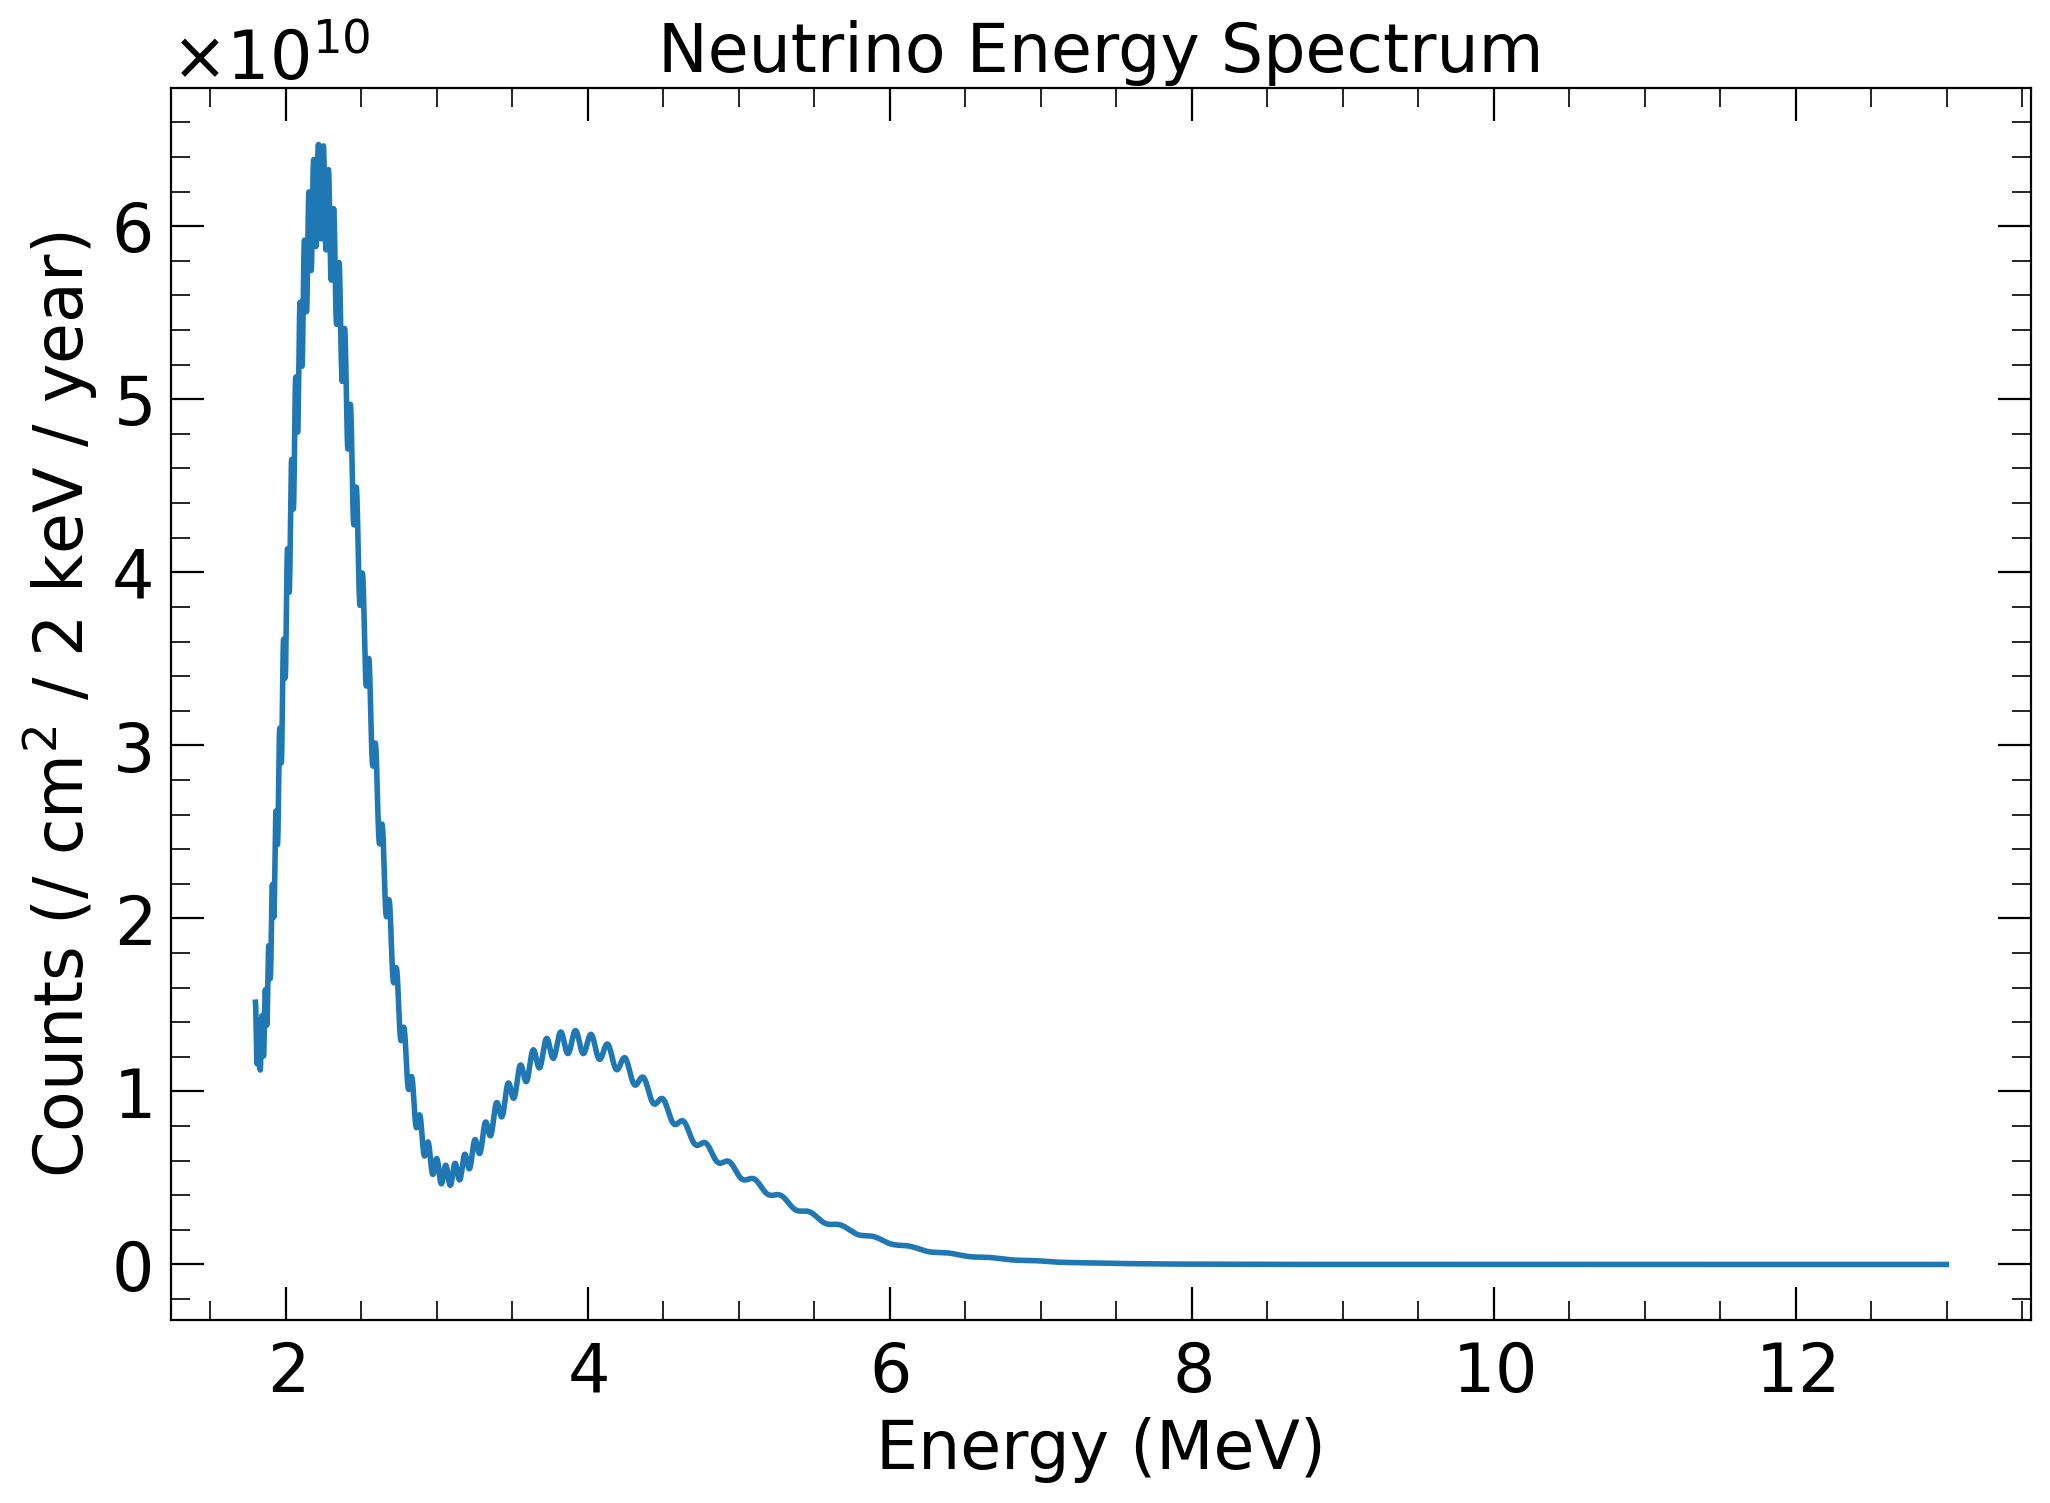
\includegraphics[width=\textwidth]{figure/reactor_nu_arr.png}
  \caption{Neutrino energy spectrum}
  \label{fig:reactor_nu_arrival}
\end{subfigure}
\hfill
\begin{subfigure}[t]{0.32\textwidth}
  \centering
  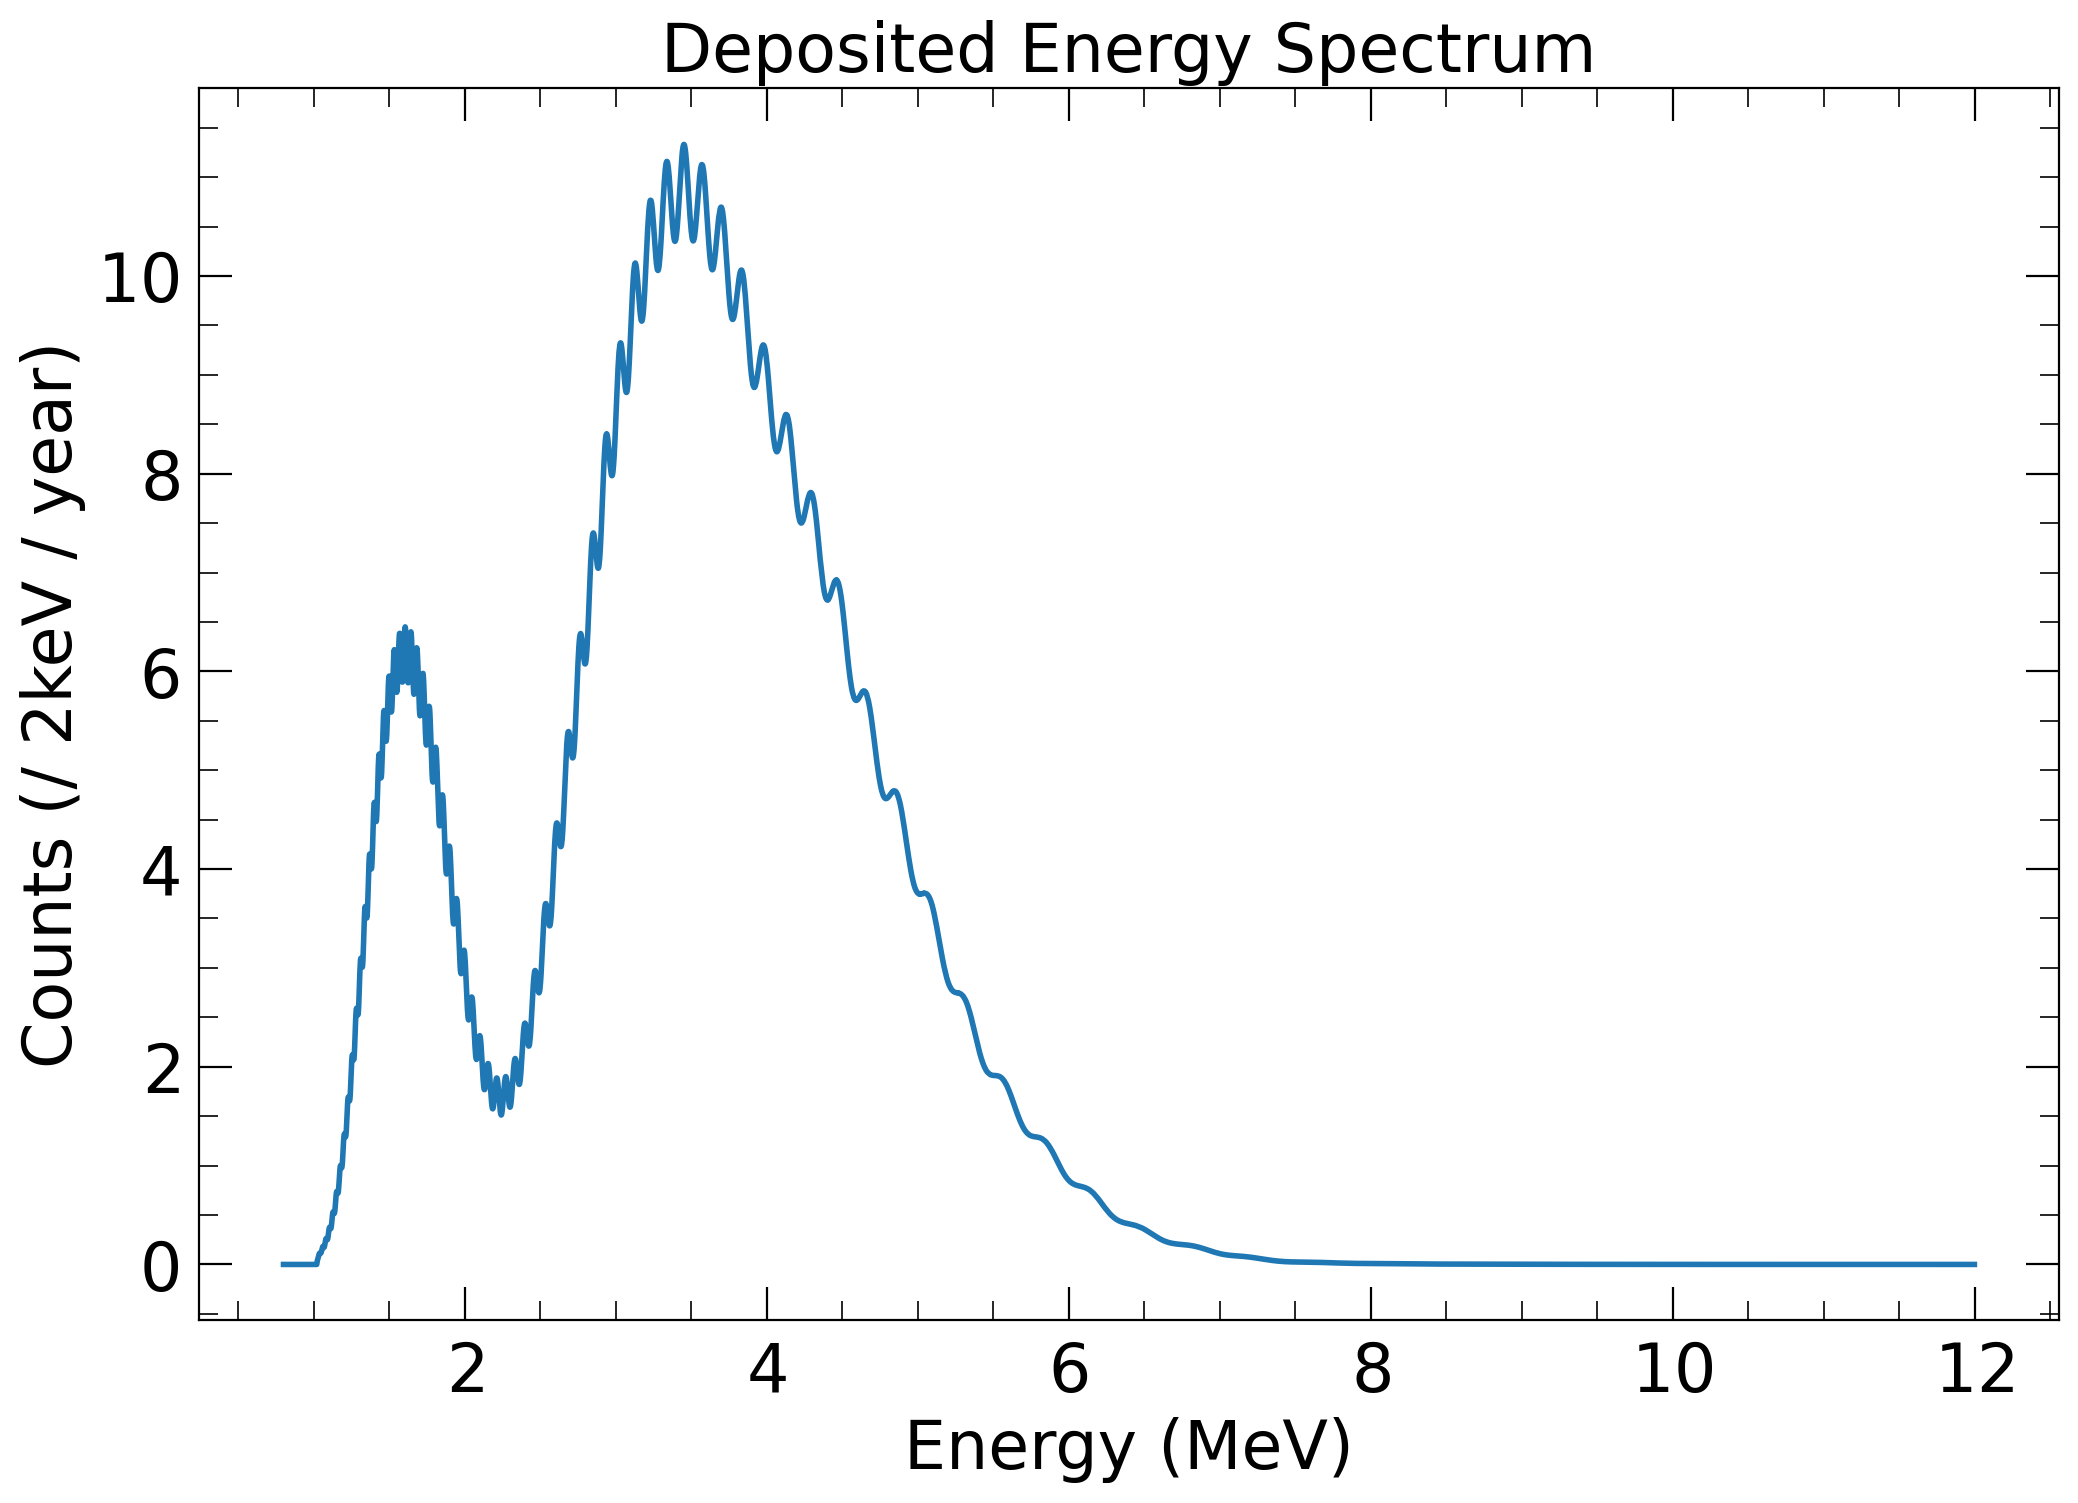
\includegraphics[width=\textwidth]{figure/depos_e_spec.png}
  \caption{Deposited energy spectrum}
  \label{fig:depo_e_spec}
\end{subfigure}
\hfill
\begin{subfigure}[t]{0.32\textwidth}
  \centering
  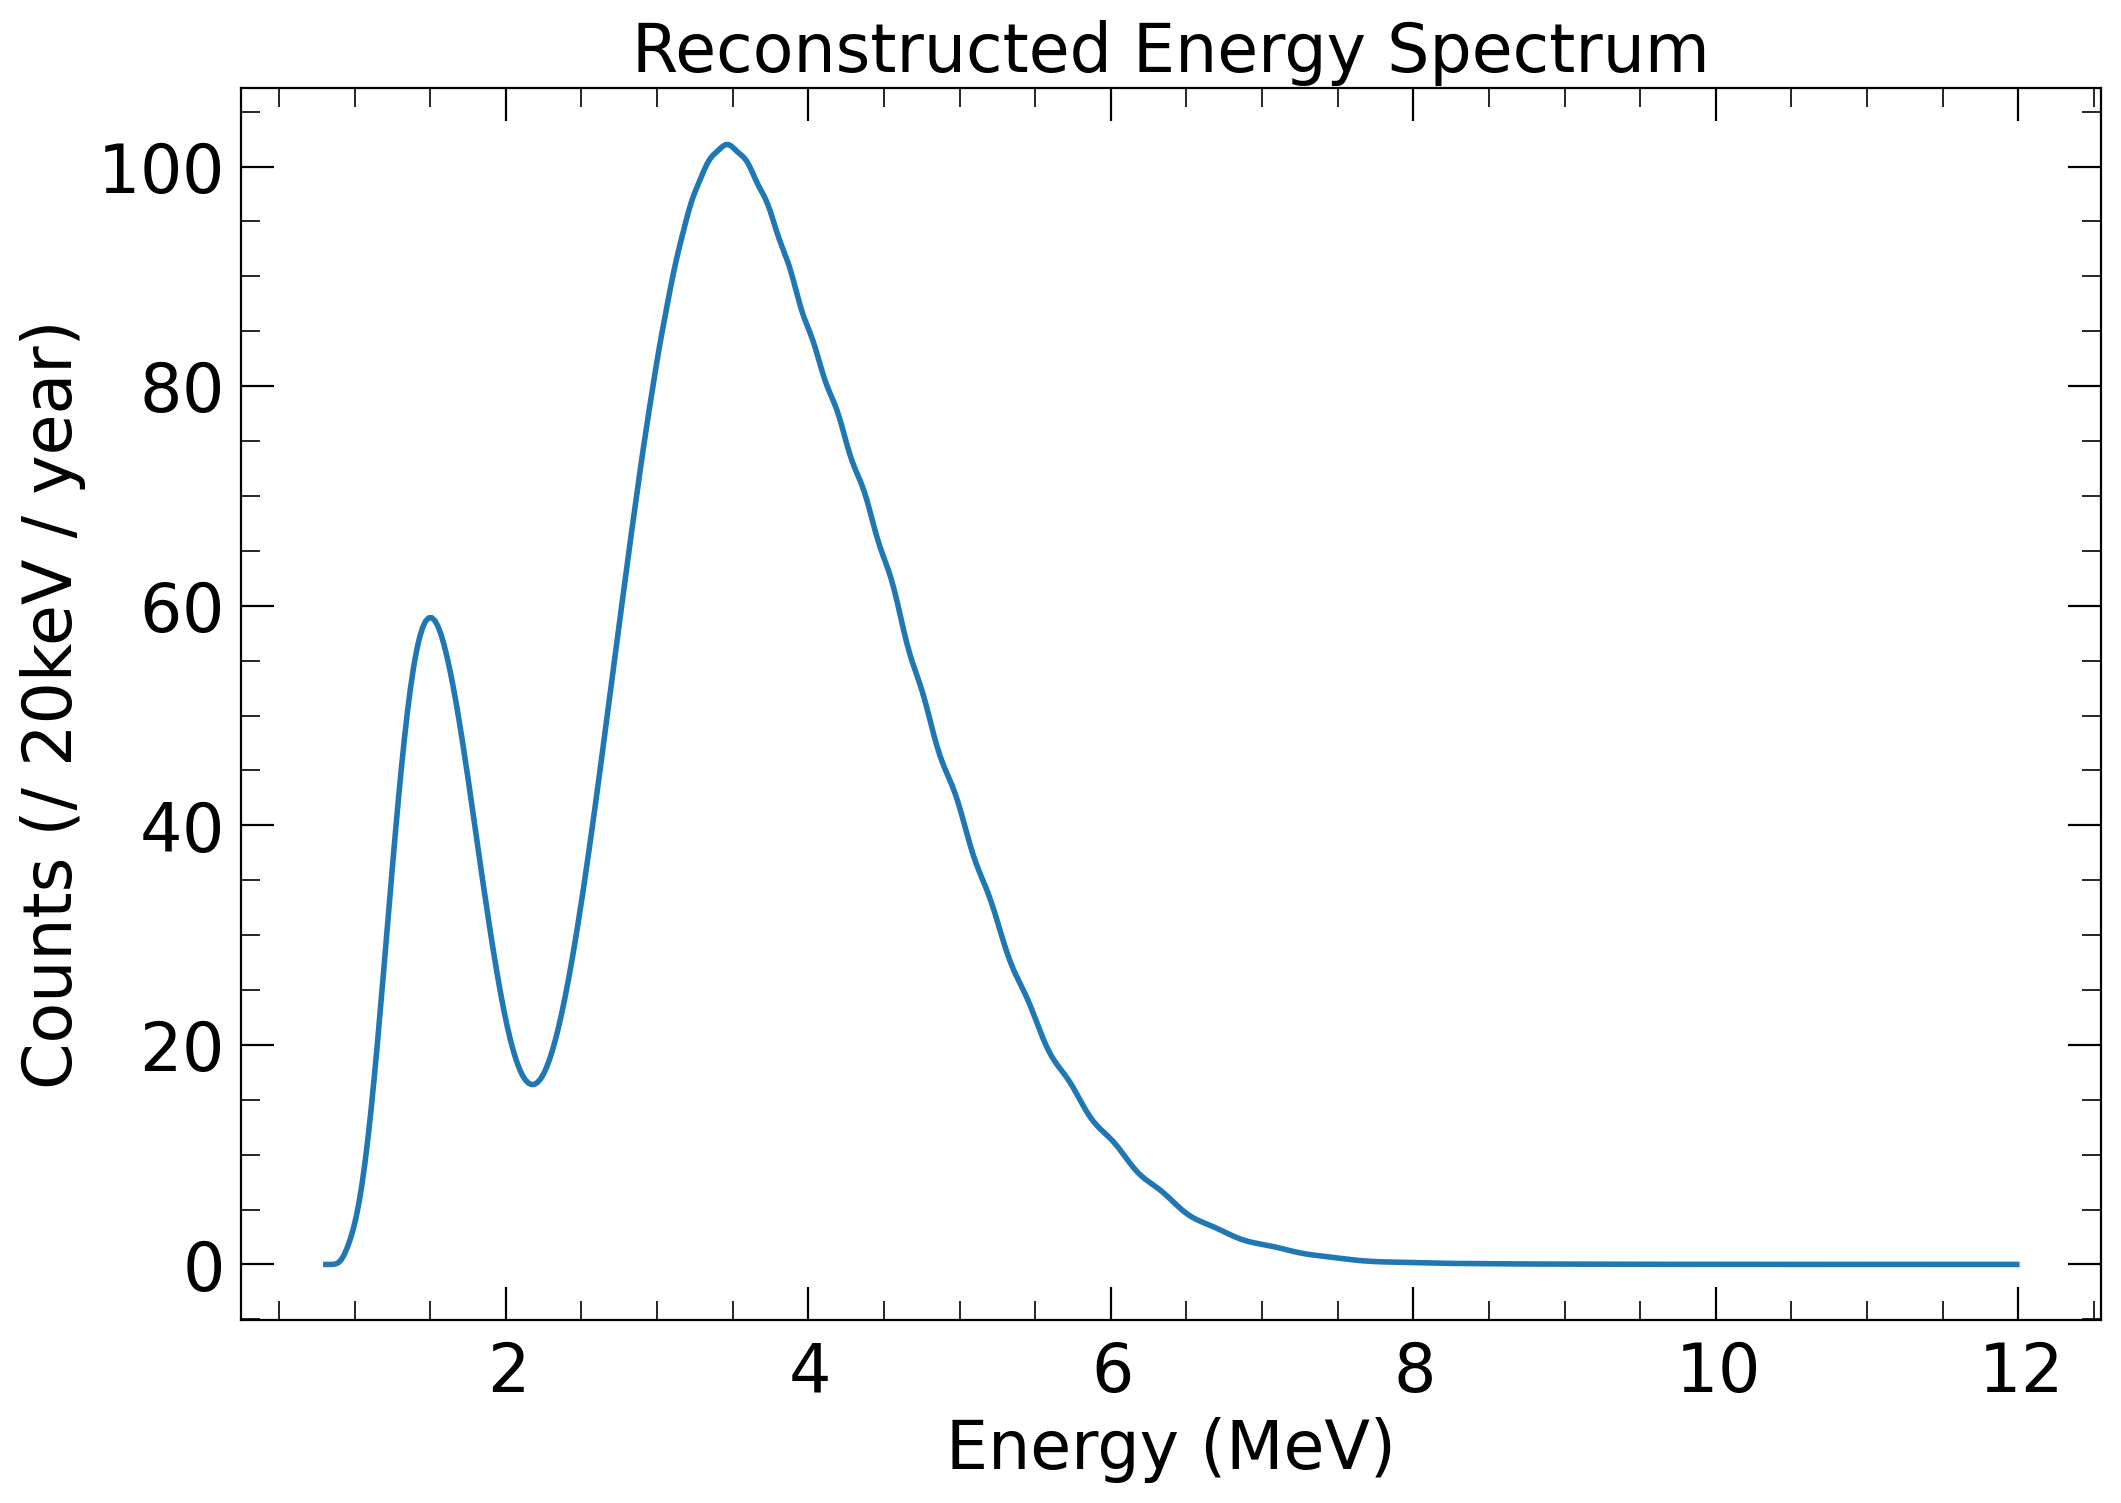
\includegraphics[width=\textwidth]{figure/recons_e_spec.png}
  \caption{Reconstructed energy spectrum}
  \label{fig:reconstructed_energy_spectra}
\end{subfigure}
\caption{(a) Neutrino energy spectrum arriving at the detector: the horizontal axis is the antineutrino energy $E_{\overline{\nu}_e}$ (MeV) and the vertical axis gives the event-rate density. (b) Deposited energy spectrum $\phi(E_{\rm dep})$: the horizontal axis is the true deposited (prompt) energy $E_{\rm dep}$ (MeV); the spectrum is obtained by folding the incident neutrino flux with the IBD differential cross section and the reaction kinematics. (c) Reconstructed energy spectrum $\Phi_{\rm rec}(E_{\rm rec})$: the horizontal axis is the reconstructed energy $E_{\rm rec}$ (MeV); this curve results from applying the detector energy nonlinearity and resolution smearing to the deposited-energy spectrum. The three panels together illustrate the forward projection from the theoretical neutrino flux to the observable reconstructed spectrum used in the spectral fit. All spectra are calculated assuming a single reactor source with a thermal power of $100\ \mathrm{GW}$ at a baseline of $150\ \mathrm{km}$. }
\label{fig:three_spectra}
\end{figure*}

\section{Statistical model}
\label{sec:statistic analysis}

\subsection{Model, covariance, and pull parameters}
\label{sec:statistic method}
To compare the experimentally measured reconstructed-energy spectrum with theoretical expectations, we perform a bin-by-bin fit using a covariance-matrix $\chi^2$ with Gaussian pull parameters~\cite{Ji2019CombinedNC}, written as
\begin{equation}
    \begin{aligned}
\chi^2 \;=\; (\mathbf{M}-\mathbf{T}(\boldsymbol{\theta},\boldsymbol{\alpha}))^{T}\,\mathbf{V}^{-1}\,(\mathbf{M}-\mathbf{T}(\boldsymbol{\theta},\boldsymbol{\alpha})) \ \;+\; \sum_k\left(\frac{\alpha_k}{\sigma_k}\right)^2 
    \end{aligned}
\end{equation}

The symbols are defined as follows:
$\mathbf{M}$: the data vector of observed counts in each reconstructed-energy bin (including IBD signal and backgrounds);  
$\mathbf{T}(\boldsymbol{\theta},\boldsymbol{\alpha})$: the predicted event counts vector, which depends on the physics parameters $\boldsymbol{\theta}$ (e.g. oscillation parameters) and nuisance (pull) parameters $\boldsymbol{\alpha}$;  
$\mathbf{V}$: the covariance matrix, encoding statistical uncertainties and bin-by-bin shape uncertainties;  $\alpha_k$ and $\sigma_k$: the $k$-th nuisance (pull) parameter and its prior uncertainty (constraint width). The term $\sum_k(\alpha_k/\sigma_k)^2$ implements the standard Gaussian prior constraints.
    
In our implementation, shape uncertainties for the signal and various backgrounds (bin-to-bin correlations) are incorporated into the covariance matrix $\mathbf{V}$. Systematic effects that primarily change normalization or can be described with a small number of degrees of freedom are introduced as explicit pull parameters $\alpha_k$.
Examples include reactor flux normalization, detector efficiency, background normalizations, energy nonlinearity, and energy resolution. By jointly minimizing $\chi^2(\boldsymbol{\theta},\boldsymbol{\alpha})$ with respect to $\boldsymbol{\theta}$ and $\boldsymbol{\alpha}$, we obtain best-fit values and uncertainties for the physics parameters. The fitted pull values also quantify the impact of systematic shifts on the result.

Systematic uncertainties can be broadly categorized into two types~\cite{Zhang2023theta13},
Rate uncertainties: These affect the overall normalization of the event spectrum and mainly arise from neutrino flux modeling, detector efficiency estimation, and background normalization.   
Shape uncertainties: These lead to differential deviations across energy bins and mainly originate from uncertainties in the reactor neutrino signal spectrum and background spectral shapes.
For parameter minimization, we use the \texttt{iminuit} optimization library and employ the MIGRAD algorithm. This algorithm is based on a quasi-Newton method and gradient-based iteration, making it efficient for local minimization. Once the minimization conditions (e.g., EDM below a set threshold) are satisfied, the algorithm converges and the iteration terminates.

\subsection{Wilks' theorem and Feldman-Cousins method}
\label{sec:statistical method}
In particle physics data analysis, the estimation of parameter confidence intervals often relies on the statistical behavior of the test statistic $\Delta \chi^2$. Wilks’ theorem~\cite{Wilks1938} offers a convenient method for constructing confidence intervals in the large-sample limit: under certain regularity conditions, or the estimation of a single parameter, the test statistic $\Delta \chi^2 = \chi^2(\delta) - \chi^2_{\min}$ approximately follows a chi-square distribution with one degree of freedom. Consequently, fixed thresholds (e.g., $\Delta \chi^2 = 1$ corresponding to a 68.27\% confidence interval) can be used to efficiently construct confidence regions.
However, the validity of Wilks’ theorem depends on the assumption of sufficiently large event statistics. In reactor neutrino experiments operating under low-statistics conditions, the event count in each bin may deviate significantly from the Gaussian regime, causing the $\Delta \chi^2$ distribution to depart from the ideal chi-square behavior. To address this, the Feldman–Cousins (FC) method can be adopted to construct confidence intervals.
The Feldman–Cousins approach constructs the distribution of the test statistic directly from a large number of toy Monte Carlo simulations~\cite{Feldman_1998}, ensuring correct coverage of the resulting confidence interval. This method is particularly suitable for cases involving bounded parameters or non-Gaussian distributions. Specifically, the procedure assumes a parameter value $\delta_i$ and then generates a large ensemble of toy data samples to construct the distribution of the test statistic (e.g., $\Delta \chi^2$). From this distribution, the critical value $\Delta \chi^2_{\text{crit}}(\delta_i)$ at a given confidence level is obtained. The parameter point $\delta_i$ is included in the confidence interval if the corresponding $\Delta \chi^2(\delta_i)$ from real data satisfies $\Delta \chi^2(\delta_i) \leq \Delta \chi^2_{\text{crit}}(\delta_i)$.

It is worth noting that constructing a full one-dimensional confidence interval using the Feldman–Cousins method requires generating toy Monte Carlo samples at many discrete parameter values $\delta_i$ to obtain a parameter-dependent confidence belt. This process is computationally expensive. Especially in analyses involving multiple nuisance parameters or higher-dimensional parameter spaces, the computational burden grows rapidly, making this one of the primary bottlenecks in high-precision statistical inference. Therefore, building an efficient and scalable energy spectrum fitting framework is essential for the statistical analysis of reactor neutrino experiments.


\section{Acceleration of the reactor-neutrino fitter}
\subsection{Acceleration motivation and objective function localization}
To identify and target performance bottlenecks in the spectrum fitting pipeline, we profiled the time consumption of a single fit. Figure~\ref{fig:time_distribution_in_one_fit} shows that spectrum calculation dominates the runtime: about 98.6\% (108.6 s) of the time is spent on spectrum calculation, while the minimizer and other overheads account for only 1.4\%(1.5 s). Hence, to achieve a substantial reduction in the total fit time, it is more effective to prioritize accelerating the spectrum calculation stage rather than the minimizer itself. Figure~\ref{fig:time_distribution_in_signal_spectrum_calculation} shows that the time is mainly consumed by the calculation of the detector response matrix and the deposited energy spectrum.

\begin{figure}[htbp]
  \centering
  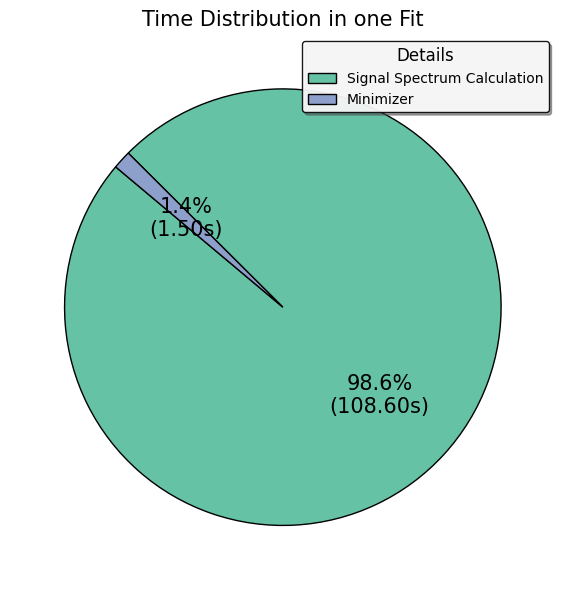
\includegraphics[width=0.4\textwidth]{figure/time_distribution_in_one_fit.png}
  \caption{Relative contributions of major processing stages in one fit. 
  The signal spectrum calculation (green) dominates the runtime, whereas 
  the minimizer (purple) accounts for only a minor share.}
  \label{fig:time_distribution_in_one_fit}
\end{figure}

\begin{figure}[htbp]
  \centering
  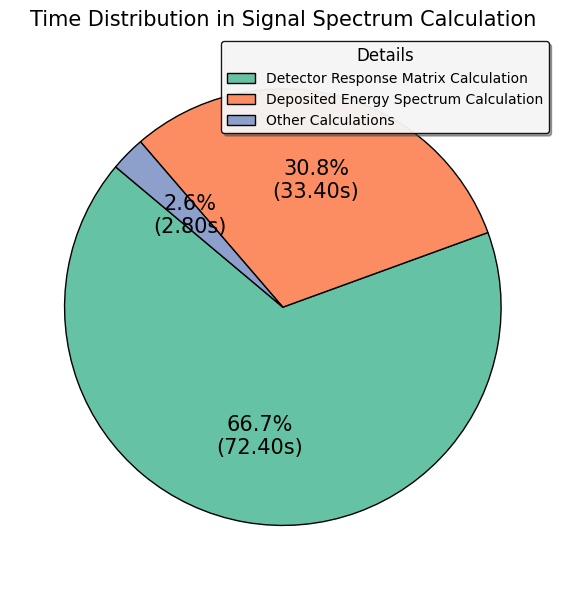
\includegraphics[width=0.4\textwidth]{figure/time_distribution_in_signal_spectrum_calculation.png}
  \caption{Internal decomposition of the signal spectrum calculation. 
  Most of the time is spent on the detector response matrix calculation (green), 
  with additional contributions from the generation of the deposited energy spectrum (orange) 
  and other minor tasks (blue).}
  \label{fig:time_distribution_in_signal_spectrum_calculation}
\end{figure}


The finer breakdown of the signal-spectrum workload reveals two hot spots:

1. Detector response matrix computation. In our implementation, this requires computing differences and normalization factors between all reconstructed-energy bin edges and visible-energy samples (roughly a $560\times5600$ array of subtraction/division operations), and evaluating the error function for each element to form the cumulative distribution function (CDF). This subtask involves both high arithmetic intensity and heavy use of special-function evaluations, and accounts for approximately 66.7\% of the spectrum time (72.4 s).
    
2. Deposited-energy spectrum calculation. The main cost here is the matrix–vector multiplication that maps neutrino energy to deposited energy using the differential cross-section (mapping) matrix, which corresponds to roughly a $5600\times5600$ matrix operation on the grid. This component contributes about 30.8\% of spectrum time (33.4 s). The remaining small contributions are negligible (2.6\%, 2.8 s).
    

Based on this profile, we focus optimization efforts on these two hot spots: (i) accelerate the detector response calculation via blocked construction of $R$ with optional $\pm 6\sigma$ truncation to reduce the number of $\operatorname{erf}$ evaluations; (ii) represent the IBD differential-cross-section matrix as a banded sparse matrix (CSR) and use sparse multiplication to skip many zero entries. In addition, we introduce caching of intermediate, parameter-independent quantities to avoid repeated evaluations.

\subsection{Caching}
In reactor neutrino spectrum fitting, the process involves extensive repeated matrix computations and nonlinear transformations, which significantly affect overall computational efficiency. To address this, we introduce a caching mechanism to reduce repeated calculations of intermediate quantities during parameter estimation and large-scale toy Monte Carlo simulations, thereby accelerating the fitting process. Specifically, caching is implemented on two main levels:

\paragraph{(1) Pre-computation and storage of static quantities:}

For quantities that remain unchanged throughout the fitting process, we precompute and load them into memory prior to the fit. These static inputs include:
\begin{enumerate}    
\item the antineutrino spectra $\phi_i(E_{\overline{\nu}_e})$ from individual fission isotopes (e.g. $^{235}$U, $^{238}$U, $^{239}$Pu, $^{241}$Pu);

\item The differential cross-section matrix $\sigma(E_{\overline{\nu}_e} \to E_{\text{dep}})$ for antineutrino-proton interactions;
    
\item The default nonlinear response curve in the detector energy response model;
    
\item Preset spectral shapes of various backgrounds (e.g., natural radioactivity, cosmogenic neutrons).
\end{enumerate}  

Caching these static quantities prior to fitting eliminates the need to reload or recompute them during each iteration, significantly reducing both I/O and CPU usage.

\paragraph{(2) Reuse of cached dynamic quantities:}

For quantities that vary with parameters during the fitting procedure—such as the predicted energy spectrum, nonlinear correction functions, or combinations involving the response matrix and nuisance parameters. Although these must be recalculated in each iteration, certain input values may repeat across iterations. To avoid redundant calculations, we implement function-level caching using Python's standard functools lru\_cache decorator. This decorator maintains a limited-size hash-based cache that stores the results of function calls. If a function is invoked again with the same inputs, the cached result is returned directly, bypassing the computation and saving significant time.

This approach proves especially effective in frequent and complex operations such as spectral convolution, matrix multiplication, and evaluation of error functions. It offers considerable performance gains in scenarios involving toy Monte Carlo generation or extensive parameter scans. In practical testing, the caching strategy reduced the overall fitting time to about one-third of the unoptimized implementation, achieving a speedup of approximately $3\times$.

Similar caching strategies have been implemented in other neutrino analysis frameworks. For example, the GooStats framework employs preloaded detector response grids to achieve over an order-of-magnitude speed improvement~\cite{Ding_2018}. The caching approach proposed in this work is highly generalizable and can be readily extended to other neutrino experiments. It is particularly well-suited for high-dimensional models, complex systematic uncertainty handling, and large-scale statistical analysis involving large-scale toy MC generation.

\subsection{Storage of the differential cross-section matrix using sparse representation}
In reactor antineutrino spectrum fitting, the transformation from neutrino energy $E_{\overline{\nu}_e}$ to deposited energy $E_{\text{dep}}$ is governed by the differential scattering cross section. This transformation can be expressed as a two-dimensional response matrix $M[i,j]$, which encodes the probability density for an antineutrino with energy $E_{{\overline{\nu}_e},j}$ to contribute to a deposited energy $E_{\text{dep},i}$ through the IBD process. Due to the kinematic constraints of the IBD reaction—especially the coupling between the positron energy and its emission angle—the matrix exhibits a clearly banded sparse structure. Non-zero elements are mostly concentrated around the diagonal, satisfying $E_{\text{dep},i} \approx E_{\overline{\nu}_e,j} - \Delta$, where $\Delta \sim 0.8$ MeV accounts for the IBD threshold and annihilation correction. This sparsity pattern is illustrated in Fig.~\ref{fig:sparse_cross_section}.

Given that most matrix elements are either exactly zero or negligibly small, we adopt the Compressed Sparse Row (CSR) format provided by PyTorch to store $M[i,j]$. This format only records the positions and values of non-zero elements, significantly reducing memory usage and avoiding redundant computations on zero entries. During spectrum prediction and fitting, this response matrix is multiplied by the neutrino flux vector $\vec{\phi}(E_{\overline{\nu}_e})$ computed under various oscillation parameters, yielding the deposited energy spectrum $S(E_{\text{dep}})$. By leveraging the sparse representation, the computational complexity of matrix–vector multiplication is reduced from $O(N^2)$ to $O(Nw)$, where $w$ is the bandwidth of non-zero elements—typically much smaller than the total number of energy bins $N$—resulting in substantial computational speedup.

Moreover, sparse matrices exhibit favorable cache locality and efficient memory bandwidth usage in GPU parallel computation, further accelerating the spectrum fitting process. Benchmark tests show that, without sacrificing numerical accuracy, this sparse representation reduces the computation time for the cross-section mapping by approximately a factor of four on our Xeon Gold 6338 setup, making it a key component in the accelerated fitting pipeline.

Similar ideas are also adopted in the ReMU framework~\cite{Koch2019}, where sparse response matrices retain only the rows containing non-zero elements, coupled with fast linear algebra operations to enhance spectral construction efficiency.

Taken together, exploiting the sparsity of the differential cross-section matrix not only reduces storage and computation demands, but also significantly improves the overall performance and scalability of neutrino spectrum fitting, particularly in high-precision, low-statistics, or large-scale toy Monte Carlo analyses.

\begin{figure}[htbp]  
\centering  
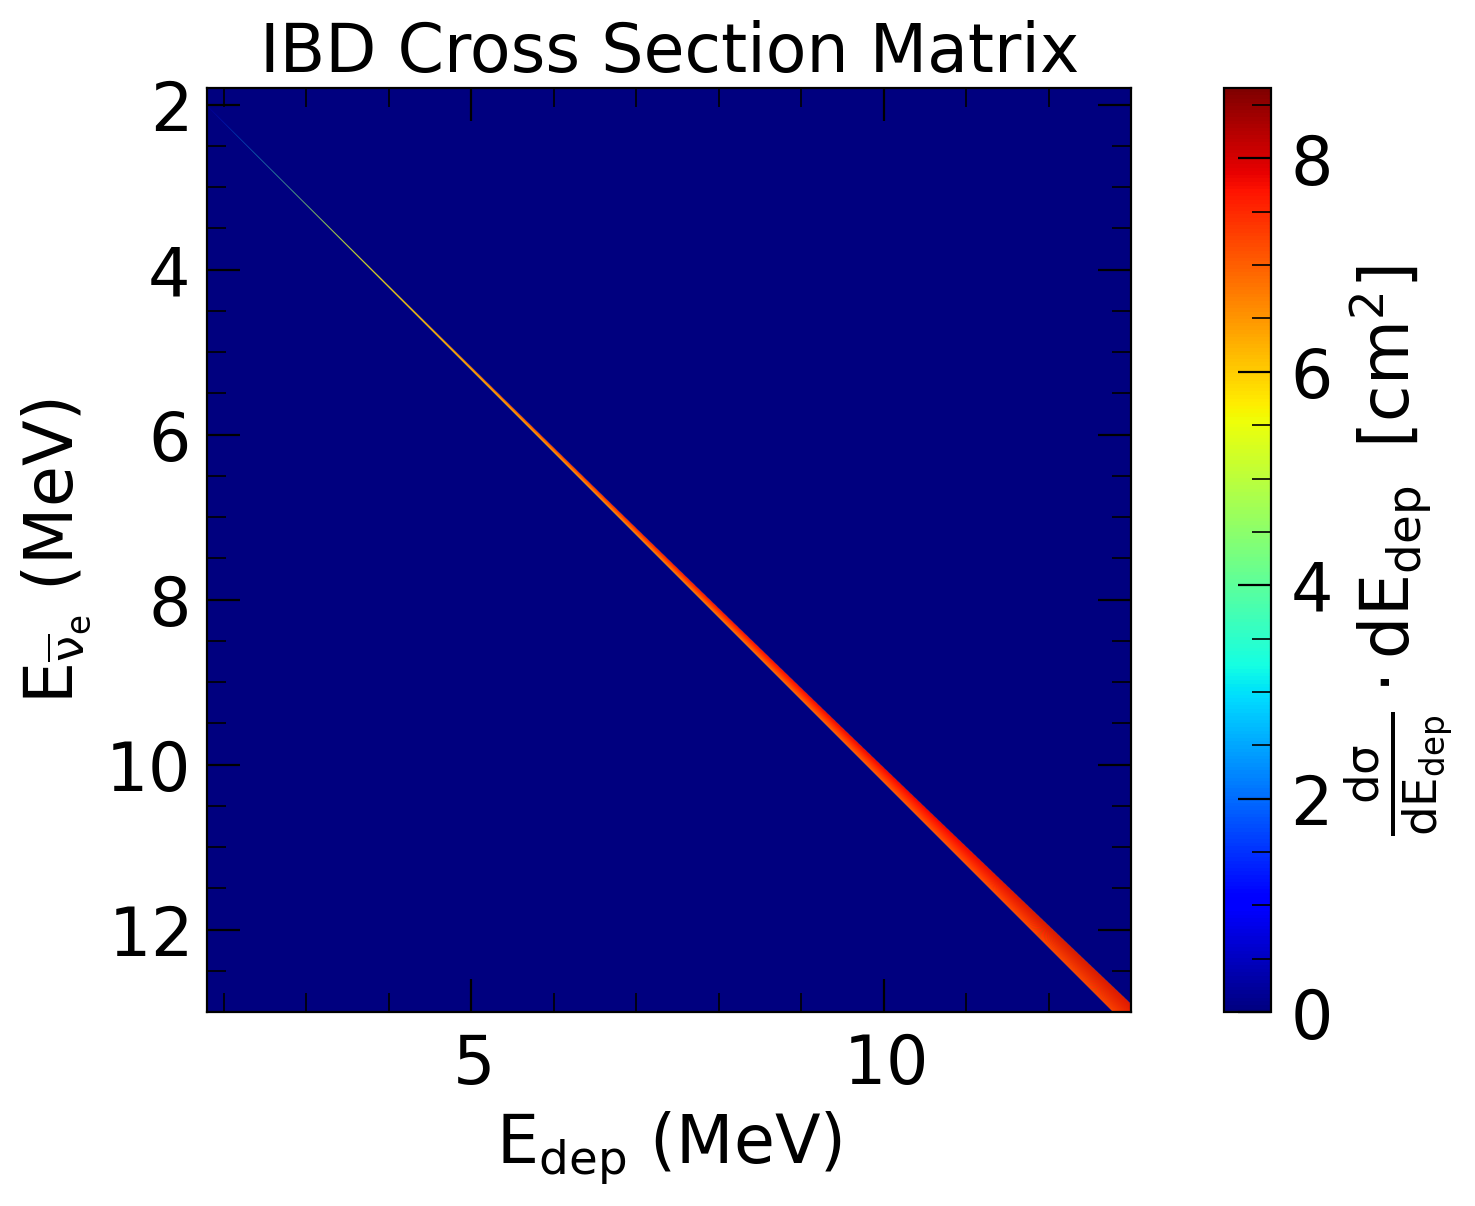
\includegraphics[width=0.4\textwidth]{figure/IBD_cross_matrix.png} 
\caption{Differential inverse beta-decay (IBD) cross-section matrix $\dfrac{\mathrm{d}\sigma}{\mathrm{d}E_{\rm dep}}(E_{\rm dep},E_{\overline{\nu}_e})$ is shown as a color map (color scale in units of $10^{-44}$ cm$^2$ per 2keV). The horizontal axis is the deposited energy $E_{\rm dep}$ (MeV) and the vertical axis is the incident antineutrino energy $E_{\overline{\nu}_e}$ (MeV); warmer colors denote larger differential cross-section values. This mapping is used to project theoretical neutrino-energy spectra into deposited-energy space for spectrum construction and fitting.}  
\label{fig:sparse_cross_section}  
\end{figure}



\subsection{Optimizing detector response matrix calculation via blocked computation}
The detector response matrix is used to map the true deposited energy of a particle to the corresponding reconstructed energy distribution. Each element of the response matrix represents the probability of mapping a given deposited energy to a reconstructed energy bin. In the traditional implementation, the response matrix is a two-dimensional array of size approximately $560 \times 5600$, with 560 bins for the reconstructed energy spectrum and 5600 bins for the deposited energy spectrum. Constructing the matrix requires computing each element individually: first performing a subtraction to determine the lower and upper energy boundaries, then dividing by the standard deviation and evaluating the error function (erf) for cumulative integration, and finally taking the difference to obtain the probability. This element-wise computation is computationally expensive, especially since the error function itself is costly to evaluate. Furthermore, constructing the entire matrix in a single step requires storing all intermediate results in memory, which leads to significant memory usage and data transfer overhead. Overall, this approach suffers from high computational complexity and large memory demands, making it a performance bottleneck. To reduce computational and memory load, the current implementation adopts a block processing strategy: the $560 \times 5600$ matrix is divided along the columns into smaller sub-blocks of size 512 \cite{Lam1991}. Specifically, only the energy bin data within one block are processed at a time, and the corresponding reconstructed energy probability distribution is computed for that block. Computation is thus confined to smaller blocks, allowing data reuse in the cache and reducing overall data movement. Once the calculation for a block is completed, the results are accumulated or concatenated to form the full response matrix. Because only one block’s probability distribution is generated at a time and immediately accumulated into the final matrix, there is no need to store intermediate results for the entire large matrix, significantly reducing peak memory usage and memory bandwidth requirements. This block computation method has shown substantial performance gains: in practice, setting the block size to 512 reduced the detector response matrix construction time from about 55 ms to about 27 ms ($\approx 2\times$ speedup). The block processing approach effectively exploits data locality, accelerates numerical operations such as the error function, and avoids excessive redundant memory I/O, thereby reducing overall runtime and resource consumption.



\section{Results}
\label{sec:result}

\subsection{Overall acceleration}
\label{sec:subresult}
In this section, we evaluate the performance improvements achieved by various optimization techniques in neutrino spectrum fitting. All benchmark tests were conducted on the same server equipped with an Intel Xeon Gold 6338 @ 2.00 GHz. We tested the following three main categories of acceleration strategies:

\begin{enumerate}  
\item Applying caching techniques  
\item Storing the differential cross-section matrix using sparse representation  
\item Optimizing detector response matrix calculation using blocked computation
\end{enumerate}

We tested the speedup achieved under each optimization strategy. Restricting the detector response element calculations to within 6$\sigma$ yielded a 1.5$\times$ speed-up with NumPy, but provided negligible gains with PyTorch when combined with other optimizations. Therefore, this restriction is not applied in our implementation. The caching technique contributed about a 3$\times$ speedup. Using sparse matrices to store the differential cross-section matrix resulted in about a 1.5$\times$ speedup. Using blocked multiplication resulted in about a 1.5$\times$ speedup. These results are shown in Fig.~\ref{fig:fit_per_t_opt}.


\begin{figure}[htbp]  
\centering  
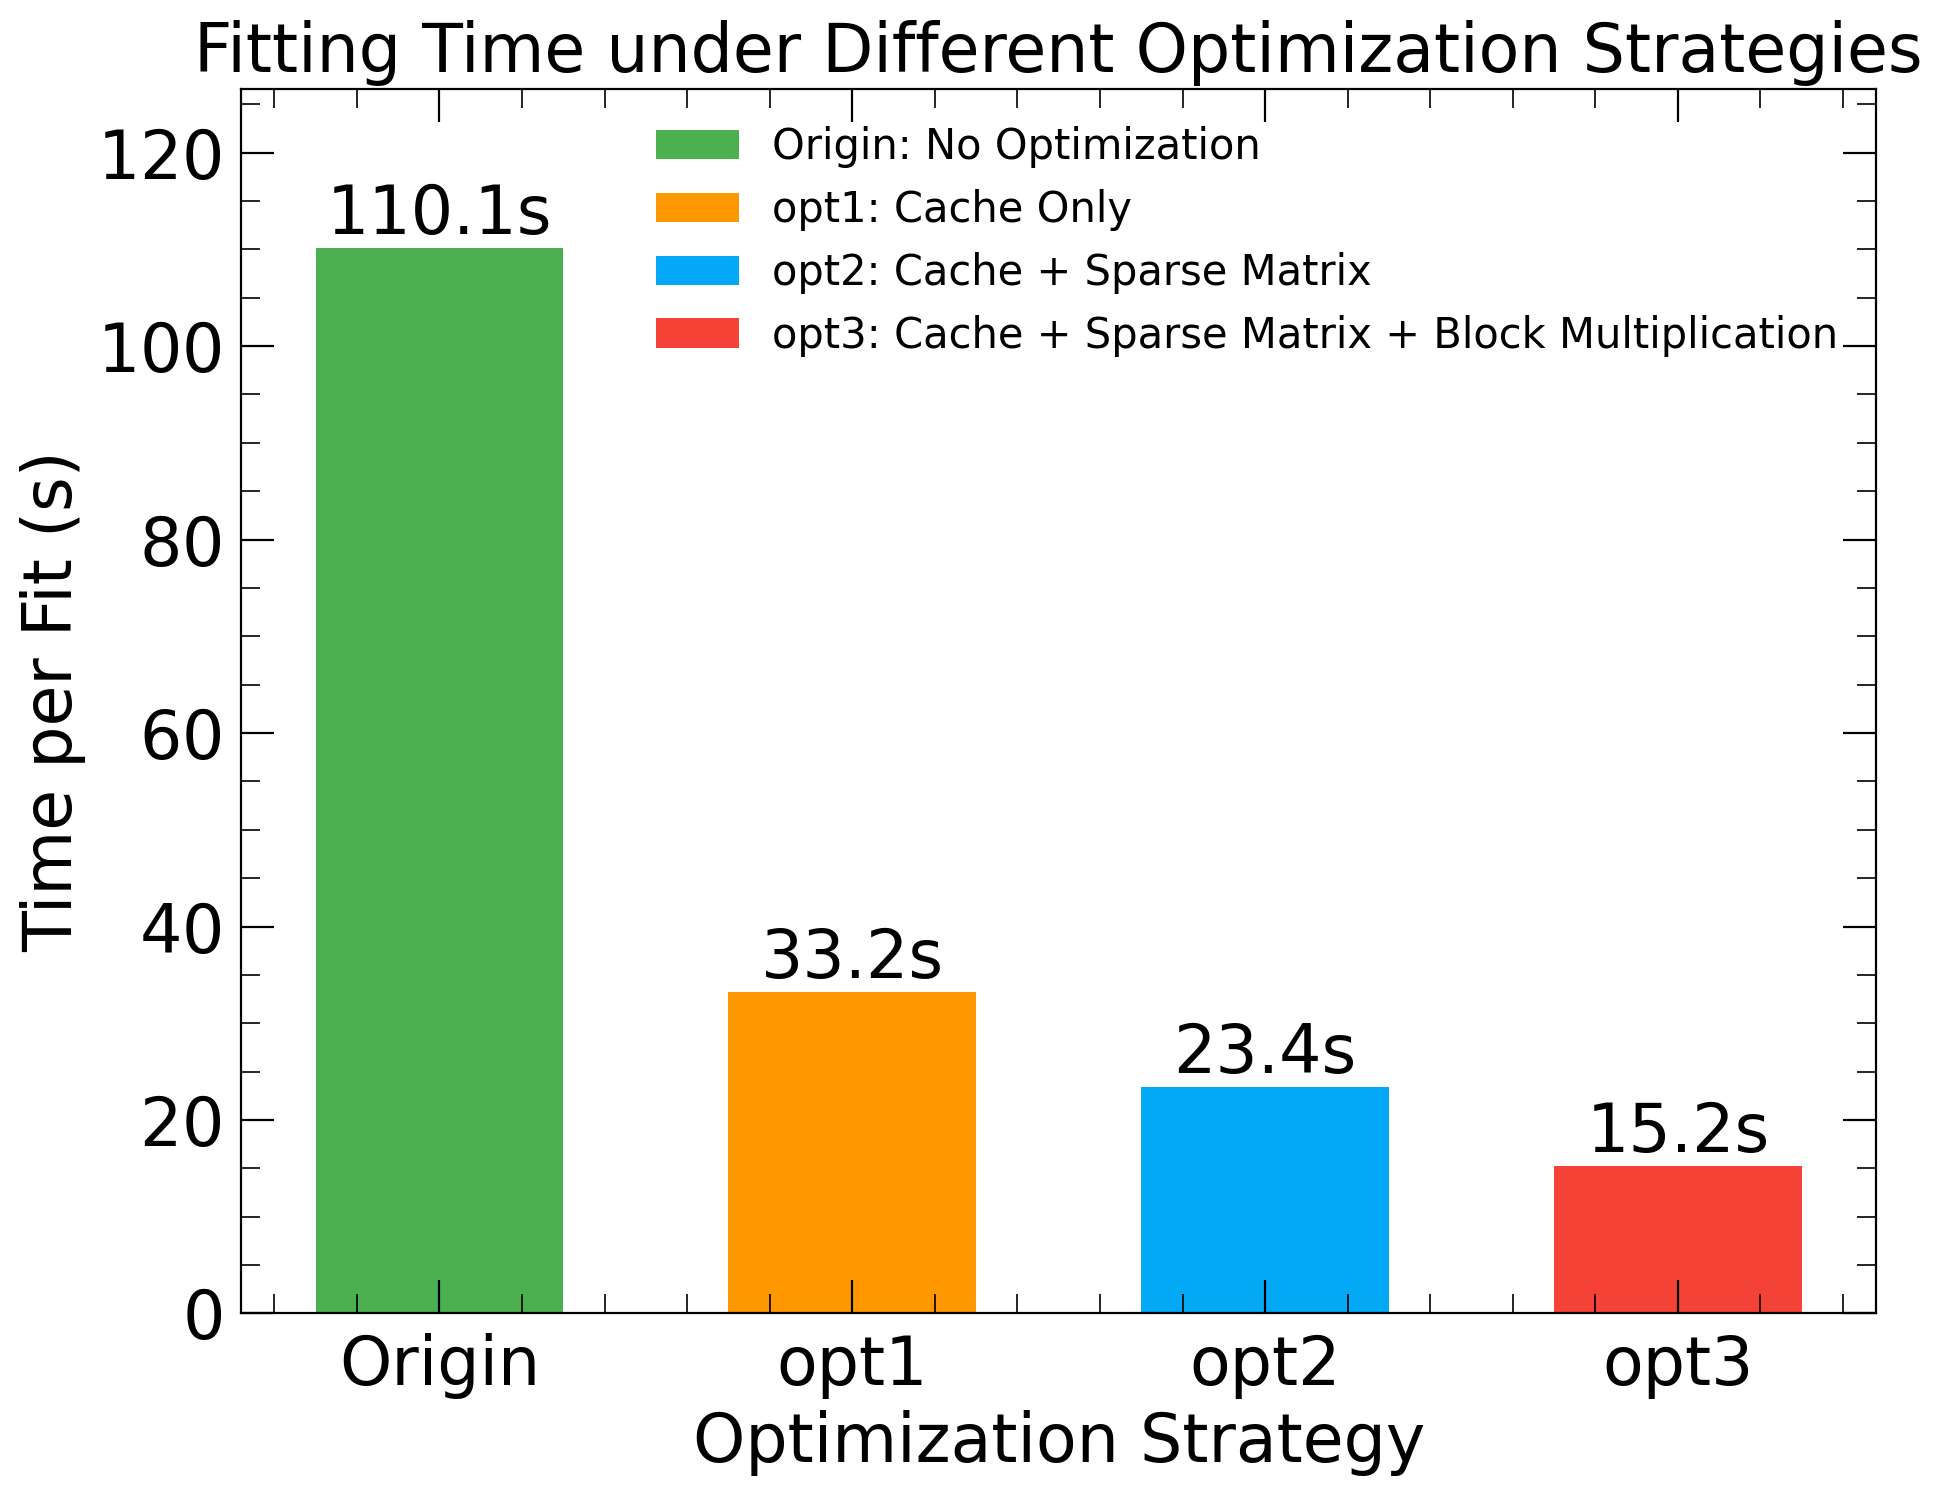
\includegraphics[width=0.4\textwidth]{figure/fitting_time_under_different_optimization_strategies.png} 
\caption{Comparison of average fitting time per fit under different optimization strategies. 
The horizontal axis lists the tested strategies: the baseline without optimization (\textit{Origin}), caching only (\textit{opt1}), caching with sparse matrix representation (\textit{opt2}), and caching with sparse matrix representation plus block multiplication (\textit{opt3}). 
The vertical axis shows the average wall-clock time in seconds required for a single fit. 
The bars illustrate the progressive reduction in runtime as successive optimizations are applied, with \textit{opt3} achieving the shortest fitting time.
}  
\label{fig:fit_per_t_opt}  
\end{figure}


Fig.~\ref{fig:time_distribution_in_one_fit_final} shows that after targeted optimizations the overall fitting performance improved markedly. The total fit time was reduced from 110.1 s to 15.2 s ($\approx 7\times$ speedup) and the time spent calculating the expected signal spectrum decreased from 108.6 s to 14.3 s (also $\approx 8\times$). Within the spectrum calculation, Fig.~\ref{fig:time_distribution_in_signal_spectrum_calculation_final} shows that the detector response–matrix computation was accelerated from 72.4 s to 8.1 s ($\approx 9\times$ speedup), and the deposited-energy spectrum (differential-cross-section mapping and matrix multiplications) was accelerated from 33.4 s to 5.0 s ($\approx 6\times$ speedup).

\begin{figure}[htbp]
\centering
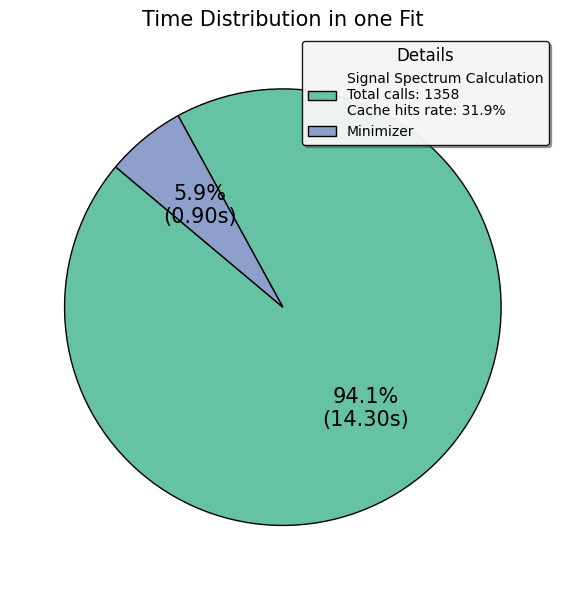
\includegraphics[width=0.4\textwidth]{figure/time_distribution_in_one_fit_final.png}
\caption{Relative contributions of major processing stages in one fit after optimization. The signal spectrum calculation (green) still dominates the runtime, but the time consumption has contracted to 14.30s.}
\label{fig:time_distribution_in_one_fit_final}
\end{figure}

\begin{figure}[htbp]
\centering
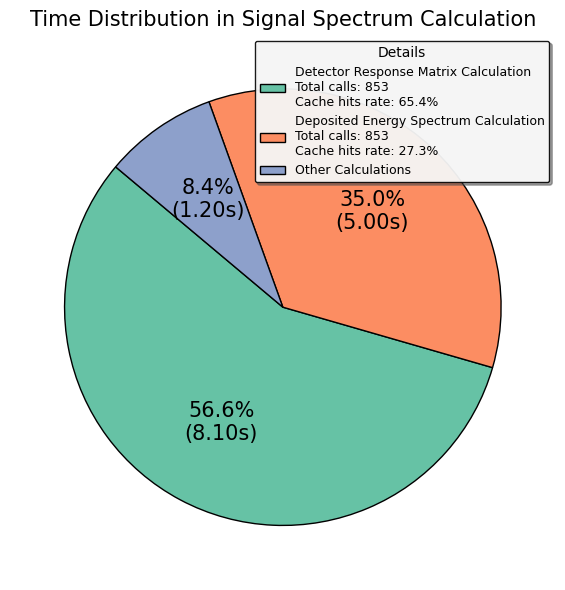
\includegraphics[width=0.4\textwidth]{figure/time_distribution_in_signal_spectrum_final.png}
\caption{Internal decomposition of the signal spectrum calculation after optimization.}
\label{fig:time_distribution_in_signal_spectrum_calculation_final}
\end{figure}


\subsection{Impact of bin width on fitting time}
\label{sec:bin}
We also studied the effect of different numbers of reconstruction energy bins on the total fitting time. Fixing the reconstructed-energy range to [0.8, 12.0] MeV, we divided the reconstructed energy into $N_{\rm bin}=560, 280, 140, 70, 35$ equally spaced bins and performed tests under the same optimization strategies. Fig.~~\ref{fig:fit_time_per_bins} shows the dependence of the total fitting time on the histogram bin width for several optimization strategies. In all cases, the fitting time decreases monotonically as the bin width increases. This trend arises because a larger bin width reduces the total number of bins in the reconstructed energy spectrum. Consequently, the dimensions of the detector response matrix shrink, lowering the computational workload per likelihood evaluation.

The tested optimization strategies—including caching, sparse matrix (CSR) representation, and block (tiled) multiplication—each provide performance improvements compared to the baseline. Caching and sparse matrix representation consistently yield speedups across the entire bin-width range. In contrast, block multiplication delivers a notable performance boost only for small bin widths, where the matrix dimensions are largest and computational complexity is highest, but offers little to no advantage for large bin widths.

In reactor antineutrino spectrum fitting, the construction and application of the detector response matrix $R$ is one of the main computational bottlenecks. Let $R$ have dimensions $M \times N$, where $M$ is the number of reconstructed-energy bins and $N$ is the number of deposited-energy bins. Each matrix element $R_{ij}$ must be evaluated via a Gaussian integral (error function $erf$) to obtain the corresponding probability. The scalar operation count for directly constructing the full matrix can therefore be approximated as
\begin{equation}
 \begin{aligned}
\text{Cost}_{\text{full}} \propto C \times M \times N,
 \end{aligned}
\end{equation}
where $C$ denotes the constant cost per element, including several floating-point subtractions, divisions, and one $erf$ evaluation. Neglecting small constant factors, the overall computational complexity scales as
\begin{equation}
 \begin{aligned}
T_{\text{full}} = \mathcal{O}(M \cdot N).
 \end{aligned}
\end{equation}
When the bin width of either the reconstructed or deposited spectrum is increased (i.e., the resolution is reduced), $M$ or $N$ will decrease accordingly. For a reconstructed energy spectrum with a fixed observation range $[E_{\min}, E_{\max}]$, doubling the bin width halves the number of bins $M$, and the total computational cost scales linearly with the number of bins. When the bin width becomes large, each computation block is already small enough to fit entirely in the CPU cache, and the cache-locality advantage of block processing is diminished. Meanwhile, the fixed overhead of block processing (function calls, memory alignment, slicing, etc.) becomes significant relative to per-block computation, offsetting the performance gains originally obtained from improved locality. Consequently, once the matrix size falls below a certain threshold (i.e., for sufficiently coarse binning), the benefits of block processing are completely masked by fixed overhead, and the actual speedup approaches zero.

In contrast, the number of fitting iterations annotated in Fig.~~\ref{fig:fit_time_per_bins} for selected points—remains nearly constant across all bin widths, indicating that the binning choice primarily affects the computational cost per iteration, rather than the convergence behavior of the minimization algorithm.

Therefore, finer binning significantly increases the size of the detector response matrix and the per-iteration computational cost, making advanced acceleration strategies essential for maintaining reasonable fitting times. For coarser binning, the inherent reduction in matrix size naturally lowers computation time, rendering block multiplication less impactful.

\begin{figure}[htbp]
  \centering
  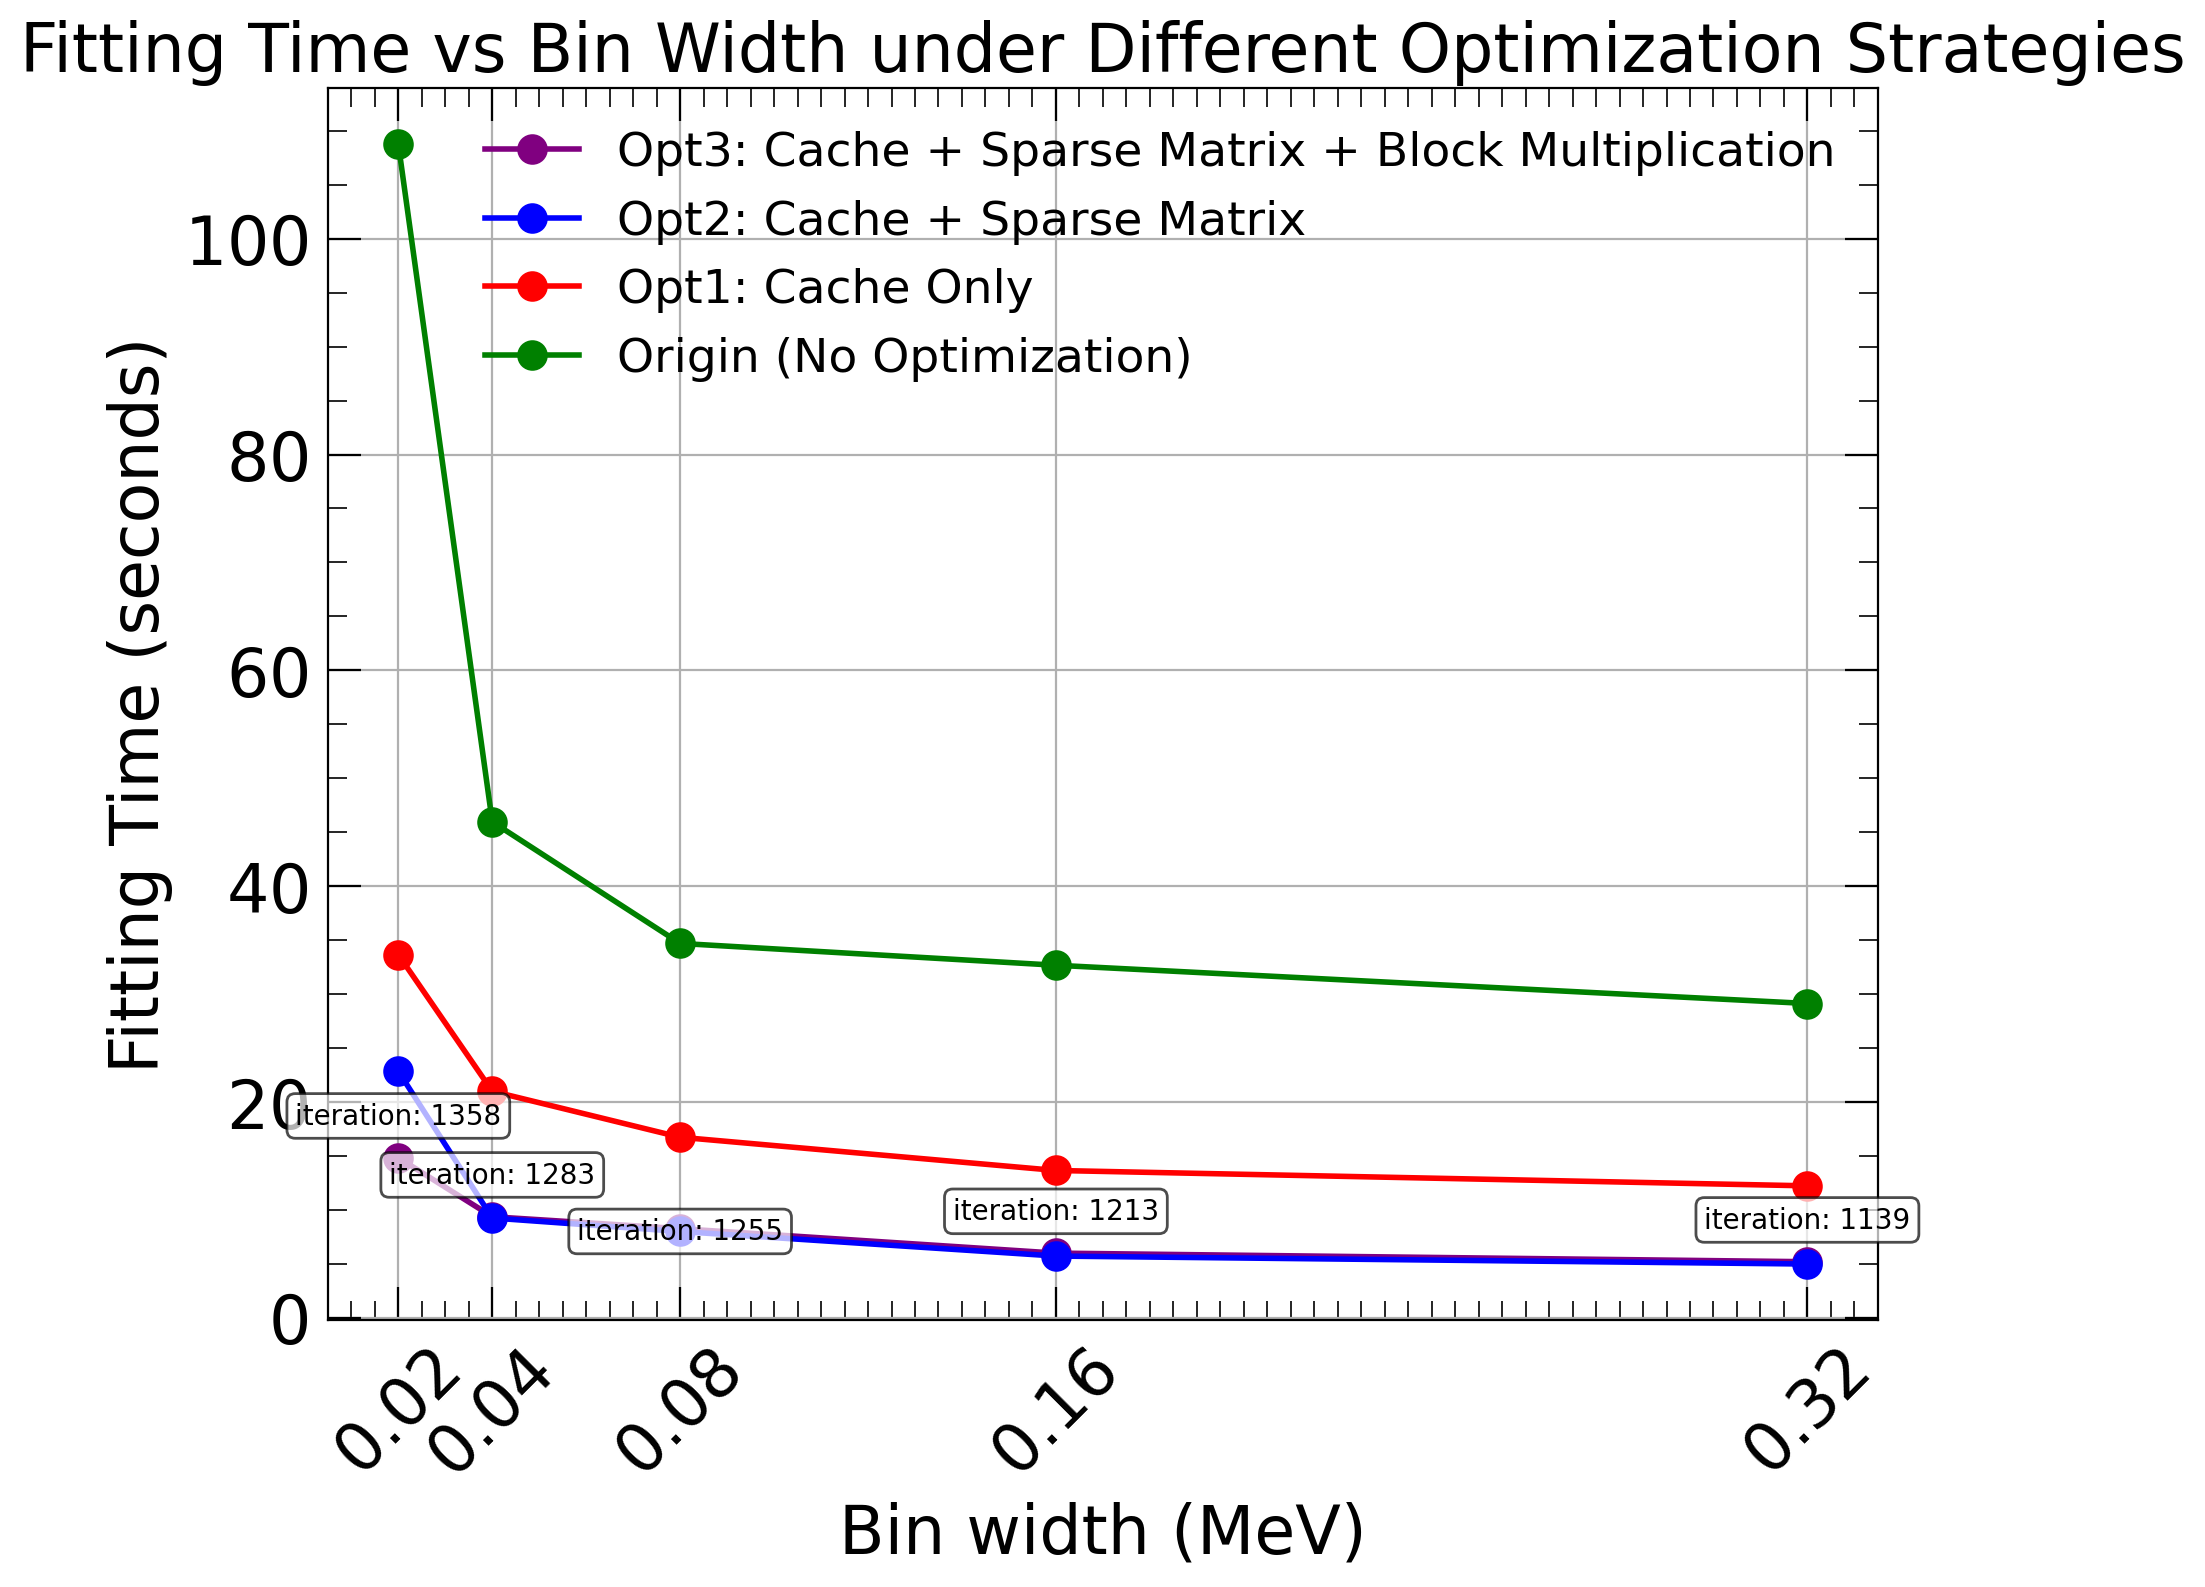
\includegraphics[width=0.4\textwidth]{figure/fitting_time_vs_bin_width.png}
  \caption{Fitting time as a function of reconstruction-bin width. The horizontal axis shows the bin width of the reconstructed-energy histogram (MeV); the vertical axis gives the total wall-clock fitting time (s) for a single full fit. Curves correspond to different optimization configurations: green — baseline (no optimization); red — caching only; blue — caching + sparse (CSR) matrix storage; magenta — caching + sparse matrix + block (tiled) matrix multiplication. Each point was obtained for the same reconstructed-energy interval ([0.8, 12.0] MeV) but with different numbers of uniform bins (equivalently different bin widths).}
  \label{fig:fit_time_per_bins}
\end{figure}


\section{Conclusions}
The acceleration techniques proposed in this study significantly improve the computational efficiency of reactor neutrino spectrum fitting while maintaining numerical accuracy. By employing caching strategies, intermediate computational results that appear repeatedly are stored and reused to avoid redundant calculations. Tests show that enabling caching leads to approximately a $3\times$ speed-up in the fitting process. By exploiting the banded sparsity of the differential cross-section or response matrices, these matrices are stored in compressed sparse formats (such as CSR), and computations are performed only on the non-zero elements. This drastically reduces the number of multiplication-addition operations and memory accesses, resulting in about a $1.5\times$ speed-up in our tests. In addition, by using blocked multiplication on the detector response matrix calculation, results in about a $1.5\times$ speed-up in our tests. When combined, these three techniques deliver an overall acceleration of $7\times$ speed-up compared to the unoptimized implementation. 

We also quantified how the choice of reconstructed-energy binning affects runtime. Increasing the bin width (equivalently reducing the number of bins) decreases the dimensions of the detector response matrix and therefore reduces the per-evaluation computational cost approximately in proportion to the matrix size; in our tests the number of minimizer iterations remained essentially unchanged, so total fit time is dominated by the cost per iteration rather than convergence properties. Practically, this implies a trade-off between spectral resolution and computational expense: very fine binning dramatically increases matrix sizes and benefits most from block multiplication, whereas caching and sparse storage produce robust speedups across a wide range of bin choices. For typical reactor-spectral analyses the combination of sparse storage and caching offers the best cost–benefit balance; tiled/block multiplication is most valuable when the response matrix is large (very fine binning).

Overall, these techniques substantially reduce the computational cost of reconstructed-energy spectrum fitting and provide an efficient, scalable framework to accelerate forward-folding analyses. The approach is broadly applicable to current and future neutrino experiments (e.g. JUNO, Hyper-Kamiokande, DUNE), enabling larger toy-MC campaigns, faster parameter scans, and more practical construction of frequentist confidence belts.

\begin{acknowledgements}
This work was supported by the National Young Talents Recruitment Program of the Chinese Academy of Sciences (Grant No. 2024000136) and the Talent Introduction Program of the Institute of High Energy Physics, Chinese Academy of Sciences (Grant No. 2023000143). We also gratefully acknowledge the IHEP computing cluster for providing extensive CPU resources used in large-scale validation studies. Finally, We thank Liangjian Wen and Zeyuan Yu for insightful comments and valuable discussions.
\end{acknowledgements}

\begin{dataavailability}
This manuscript has no associated data. [Author’s comment: Data sharing not applicable to this article as no datasets were generated or analysed during the current study.]
\end{dataavailability}

\begin{codeavailability}
Code/software will be made available on reasonable request. [Authors’ comment: The code/software generated  during the current study is available from the corresponding author on reasonable request.]
\end{codeavailability}



% BibTeX users please use one of
\bibliographystyle{spphys}   % EPJC 用的物理风格
\bibliography{biblio}        % 这里写你的 biblio.bib 文件名（不要加 .bib）

\end{document}
